% !TEX root = ../../main.tex

% --------------------------------------
% labels: \label{mil1:res:[type]:[name]}
% --------------------------------------
% Past tense


The familiar plot of the density parameters as functions of the logarithmic scale factor is presented in~\cref{mil1:res:fig:density_params} together with markings of important milestones in the history of the universe (see~\cref{mil1:res:tab:time_of_events}). 

\begin{figure}[!ht]
    \centering
    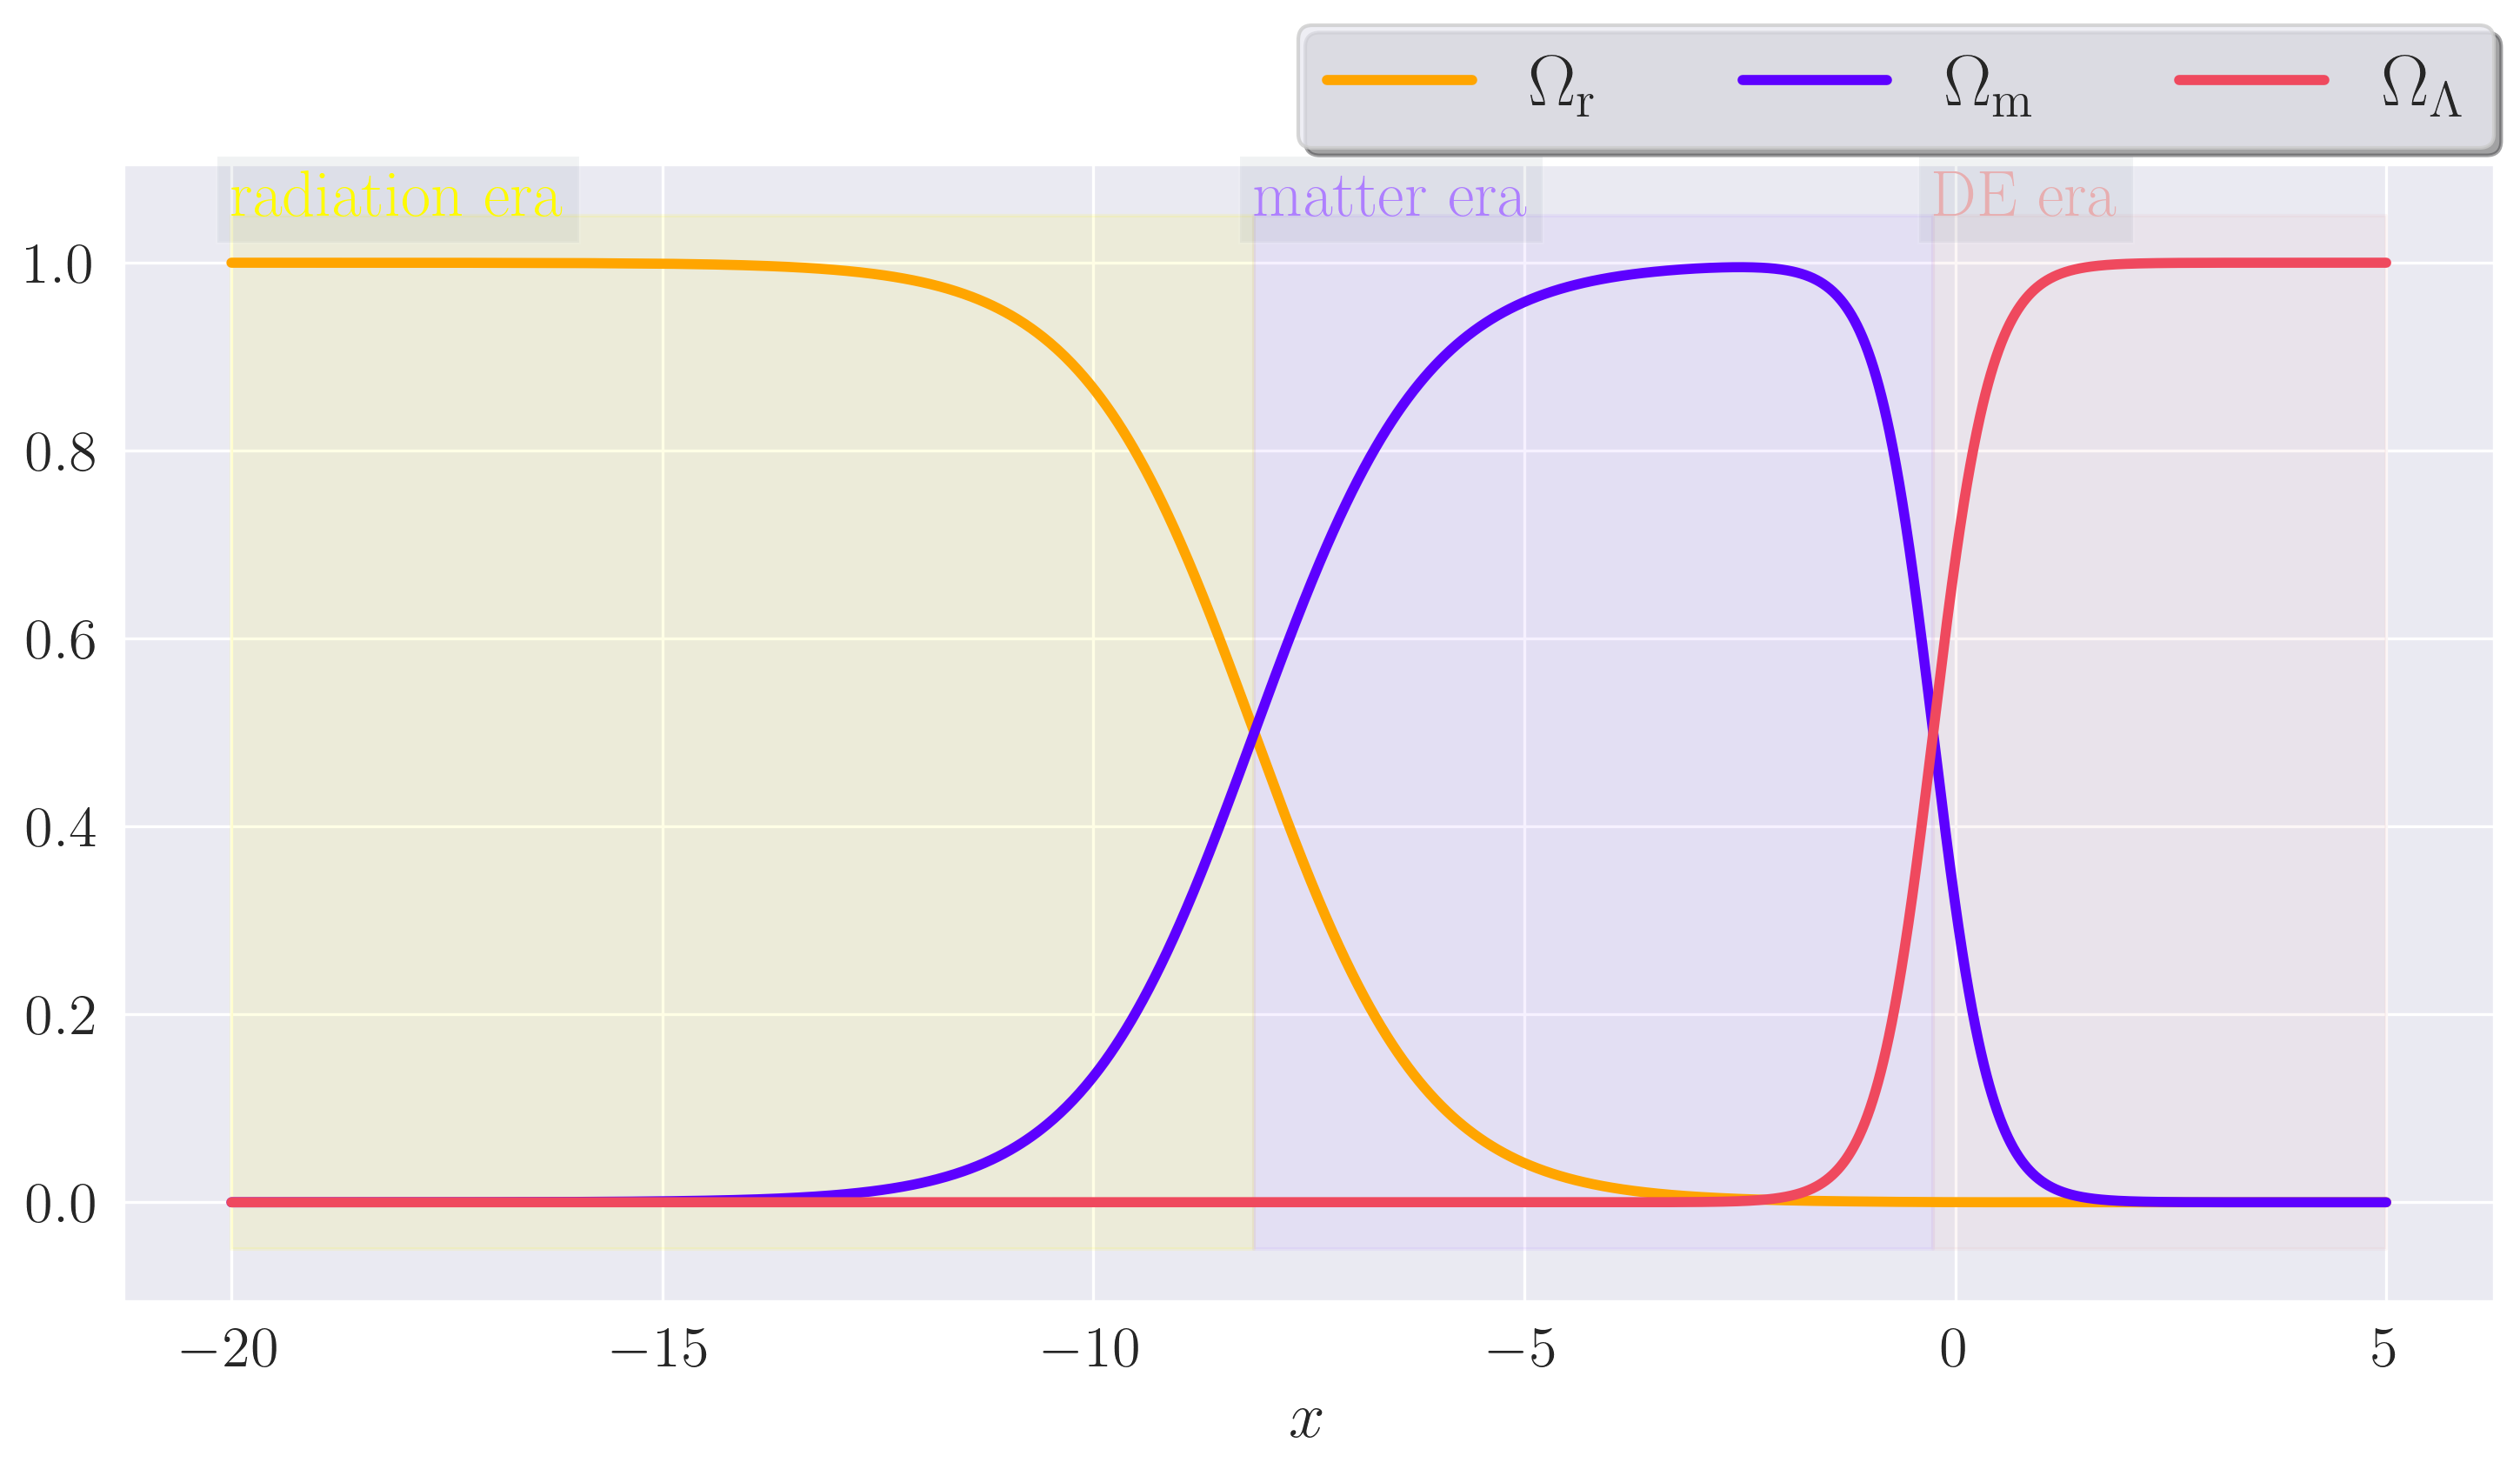
\includegraphics[width=\linewidth]{milestone1/density_params.png} 
    \caption{The graphs show the evolution of the total matter density $\OmgM[](x)$, the total radiation density $\OmgR[](x)$ and the dark energy density $\OmgL[](x)$. The era of radiation ($x<x_\mathrm{eq}$), matter ($x_\mathrm{eq}<x < x_\Lambda$) and cosmological constant ($x>x_\Lambda$) domination are marked in yellow, purple and red, respectively.} 
\label[fig]{mil1:res:fig:density_params}
\end{figure}

The conformal Hubble factor and its derivatives are presented in~\cref{mil1:res:fig:tests_hubble} over-plotted with analytical predictions from the different eras (\cref{app:hubble_derivatives:tab:eras_approx}). In the same figure you will find the product of the conformal time and Hubble factor. 


\begin{figure}
    \begin{subfigure}{\linewidth}
        \centering
        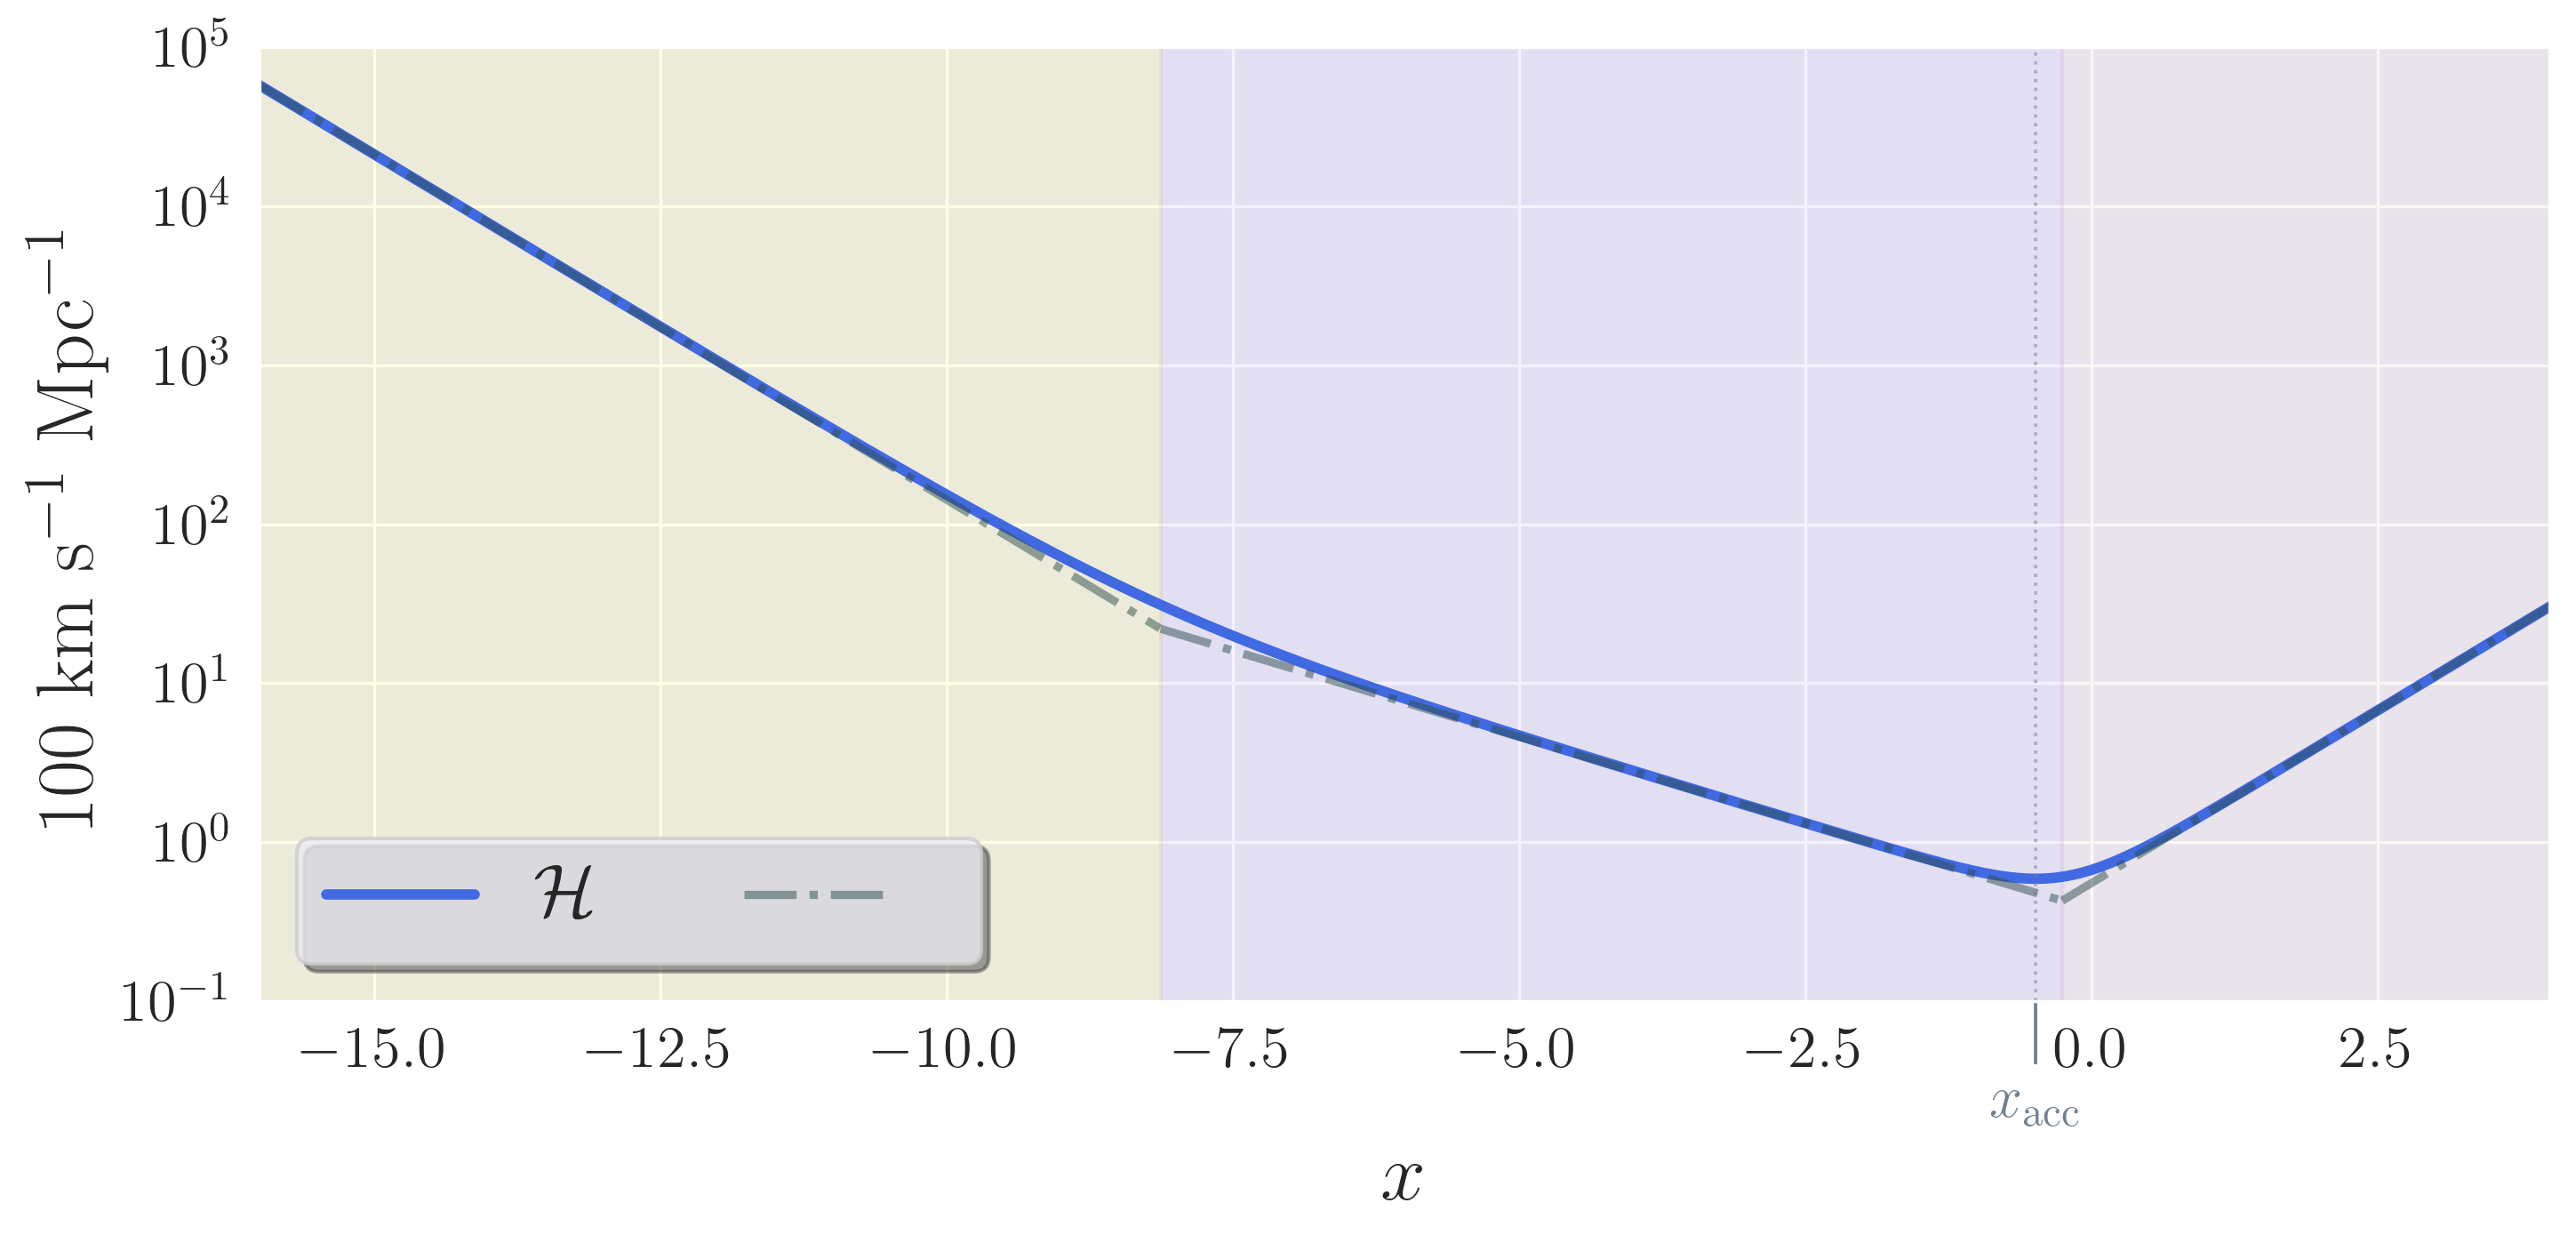
\includegraphics[width=\linewidth]{milestone1/hubble_param.png} 
        \caption{The conformal Hubble factor $\Hp(x)$. The over-plotted dash-dotted line is the corresponding analytical estimate.}
    \label[fig]{mil1:res:fig:hubble_of_x}
    \end{subfigure}
    \begin{subfigure}{\linewidth}
        \centering
        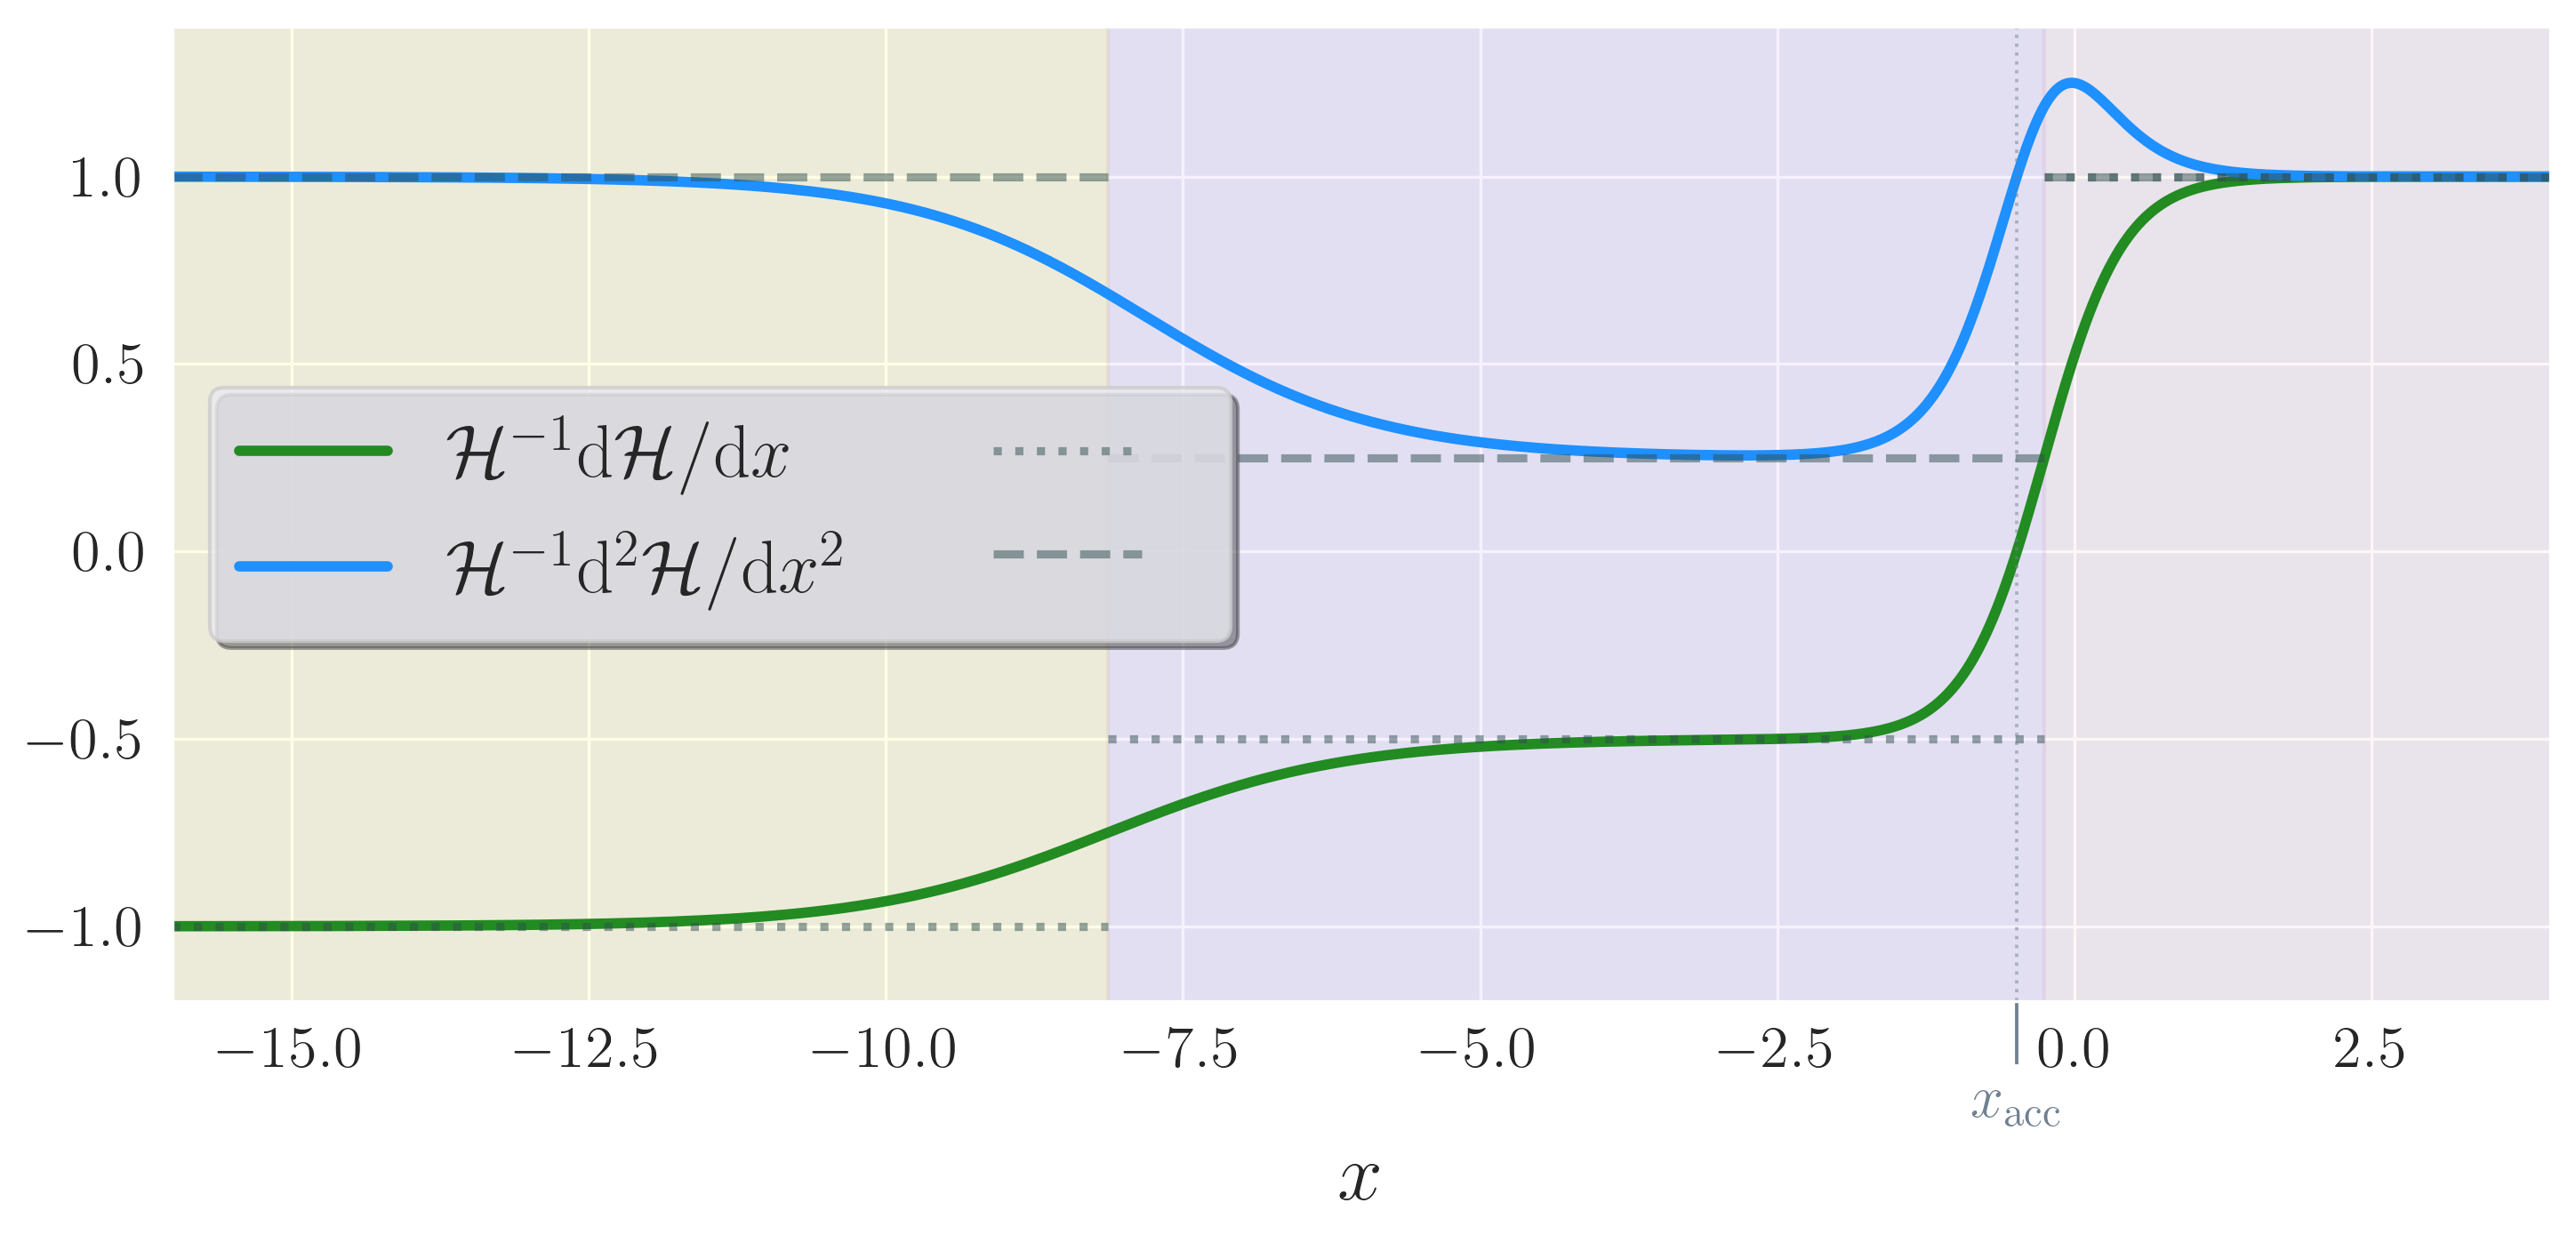
\includegraphics[width=\linewidth]{milestone1/Hubble_derivatives.png} 
        \caption{The single and double derivative of the conformal Hubble factor, scaled with the factor itself, $\frac{1}{\Hp(x)}\dv{\Hp(x)}{x}$ and $\frac{1}{\Hp(x)}\dv[2]{\Hp(x)}{x}$. The over-plotted dotted and dashed lines are the analytical estimates to the first and second derivative, respectively.} 
    \label[fig]{mil1:res:fig:der_hubble}
    \end{subfigure}
    \begin{subfigure}{\linewidth}
        \centering
        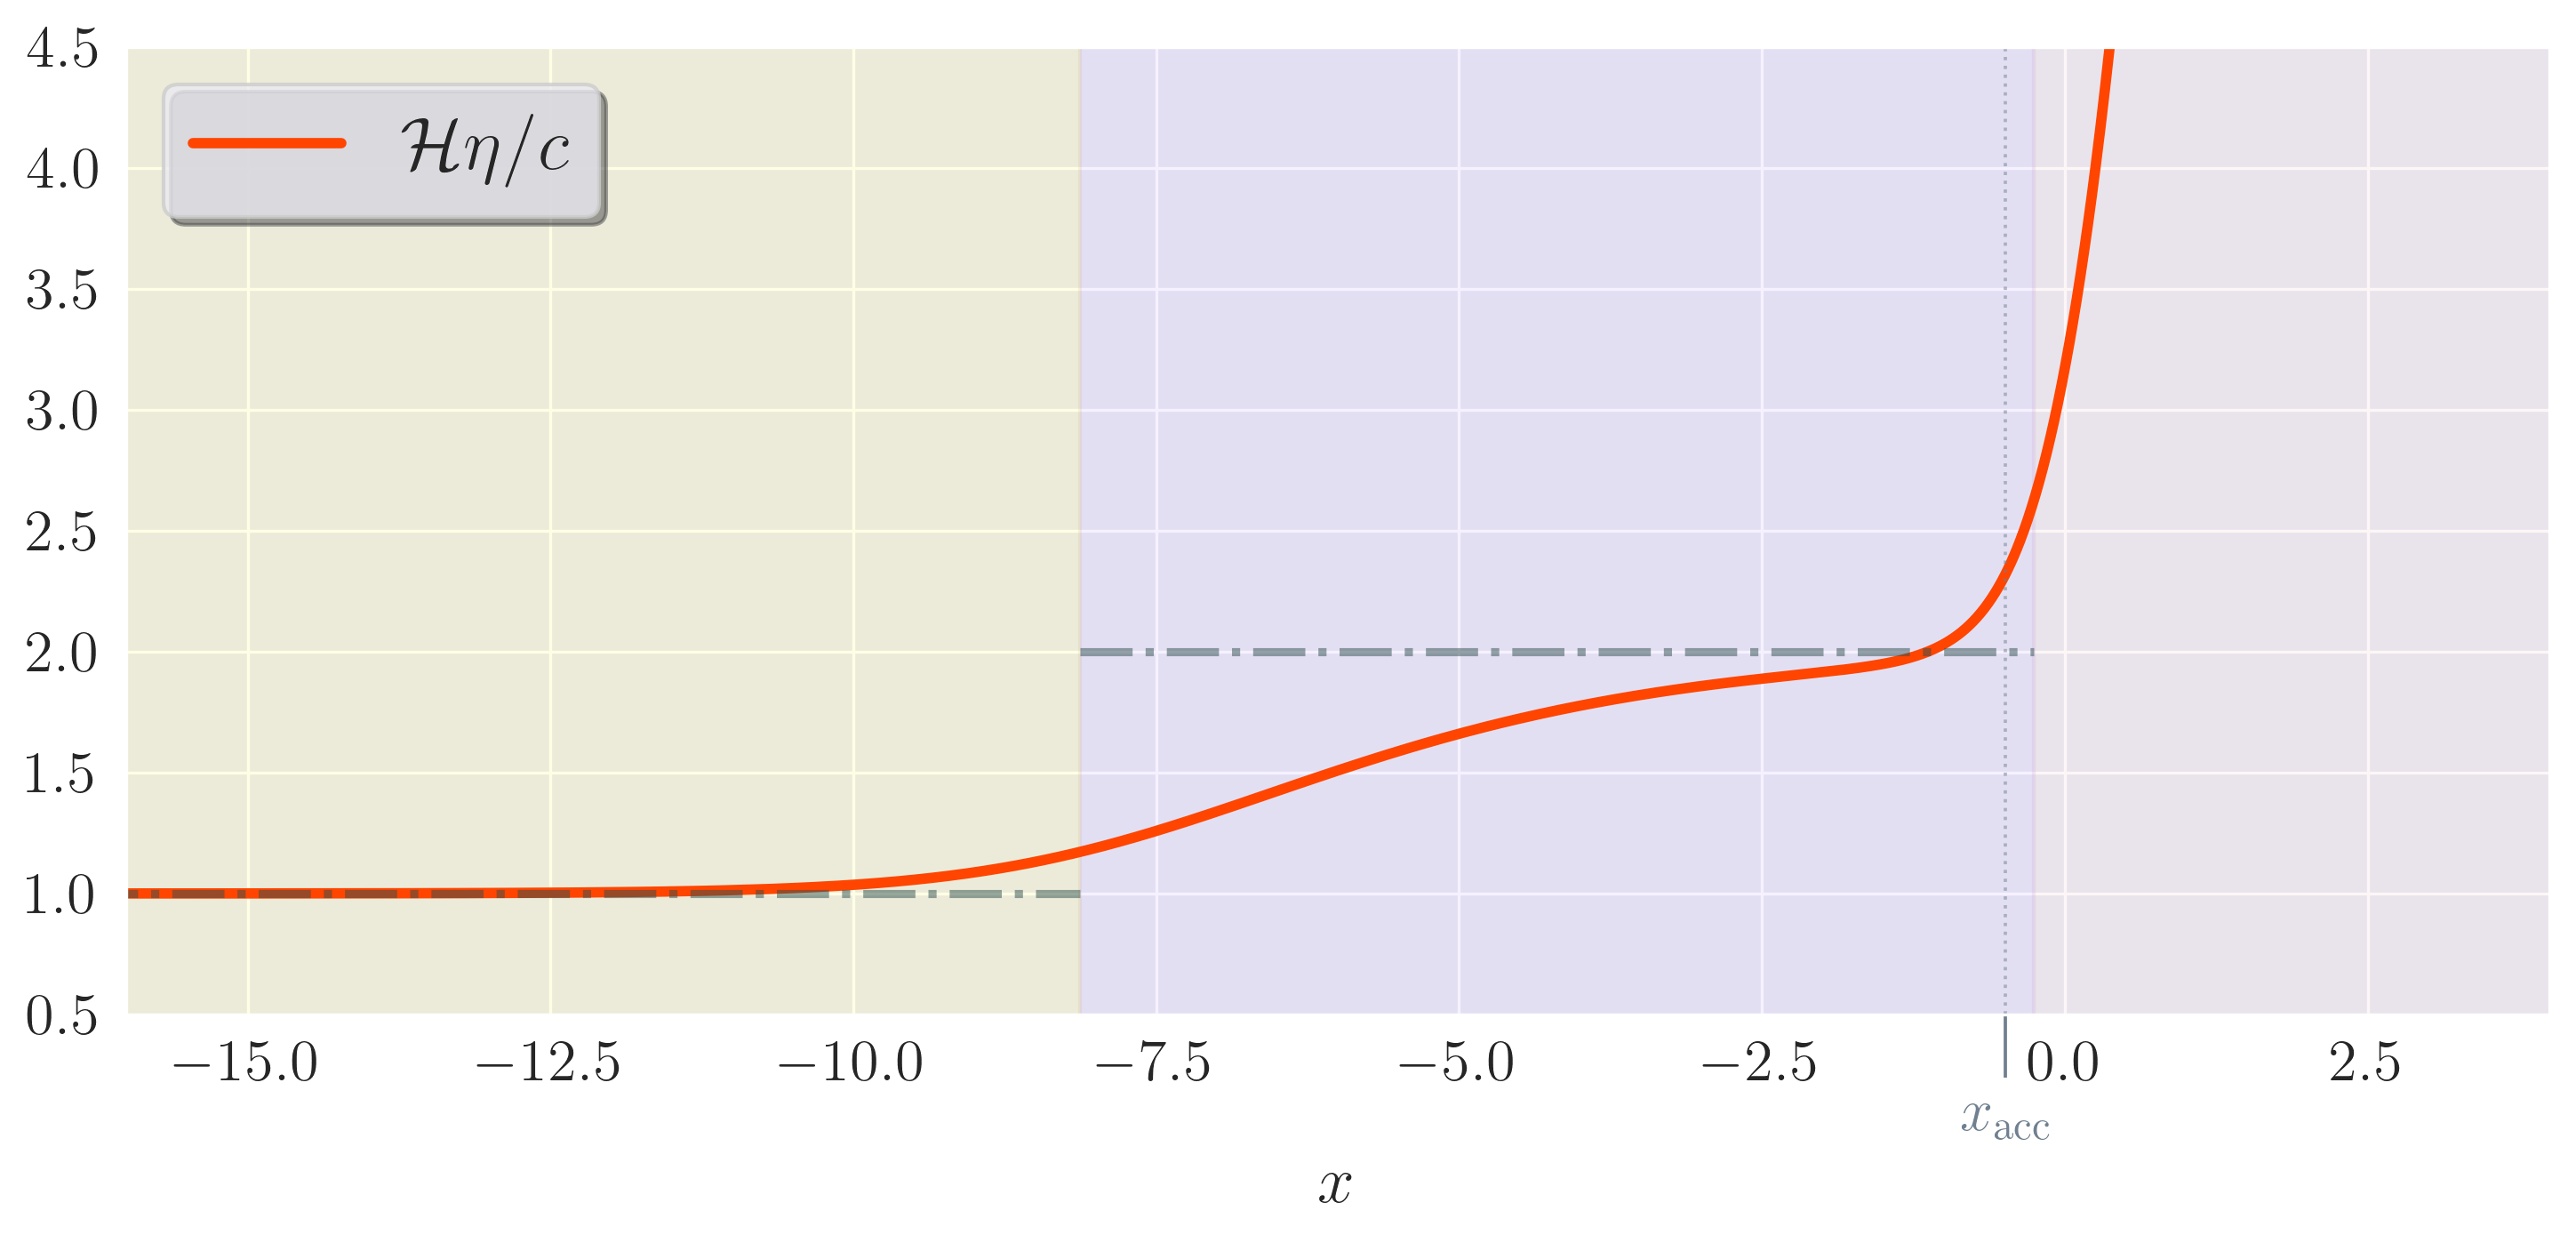
\includegraphics[width=\linewidth]{milestone1/eta_Hubble.png} 
        \caption{The product of the conformal time and Hubble factor, divided by the speed of light, $\Hp(x)\frac{\eta(x)}{c}$. The solid graph blows up at late times. The over-plotted dash-dotted line is the corresponding analytical estimate (for single-substance universe).} 
    \label[fig]{mil1:res:fig:eta_hubble}
    \end{subfigure}
    \caption{Plots demonstrating quantities related to the conformal Hubble parameter $\Hp(x)$ and the conformal time $\eta(x)$ as functions of logarithmic scale factor $x$. The dashed and/or dotted graphs are the predictions from~\cref{app:hubble_derivatives:tab:eras_approx}, i.e.~what we expect in each era (indicated by different background colours, following~\cref{mil1:res:fig:density_params}) if all non-prevailing constituents can be neglected. The beginning of acceleration is indicated by a humble vertical line.}
\label[fig]{mil1:res:fig:tests_hubble}
\end{figure}

The relationship between the cosmic and conformal time is demonstrated in~\cref{mil1:res:fig:conformal_cosmic_time}, both quantities given in gigayears (``giga-annum'' (Ga)). 

\begin{figure}[!ht]
    \centering
    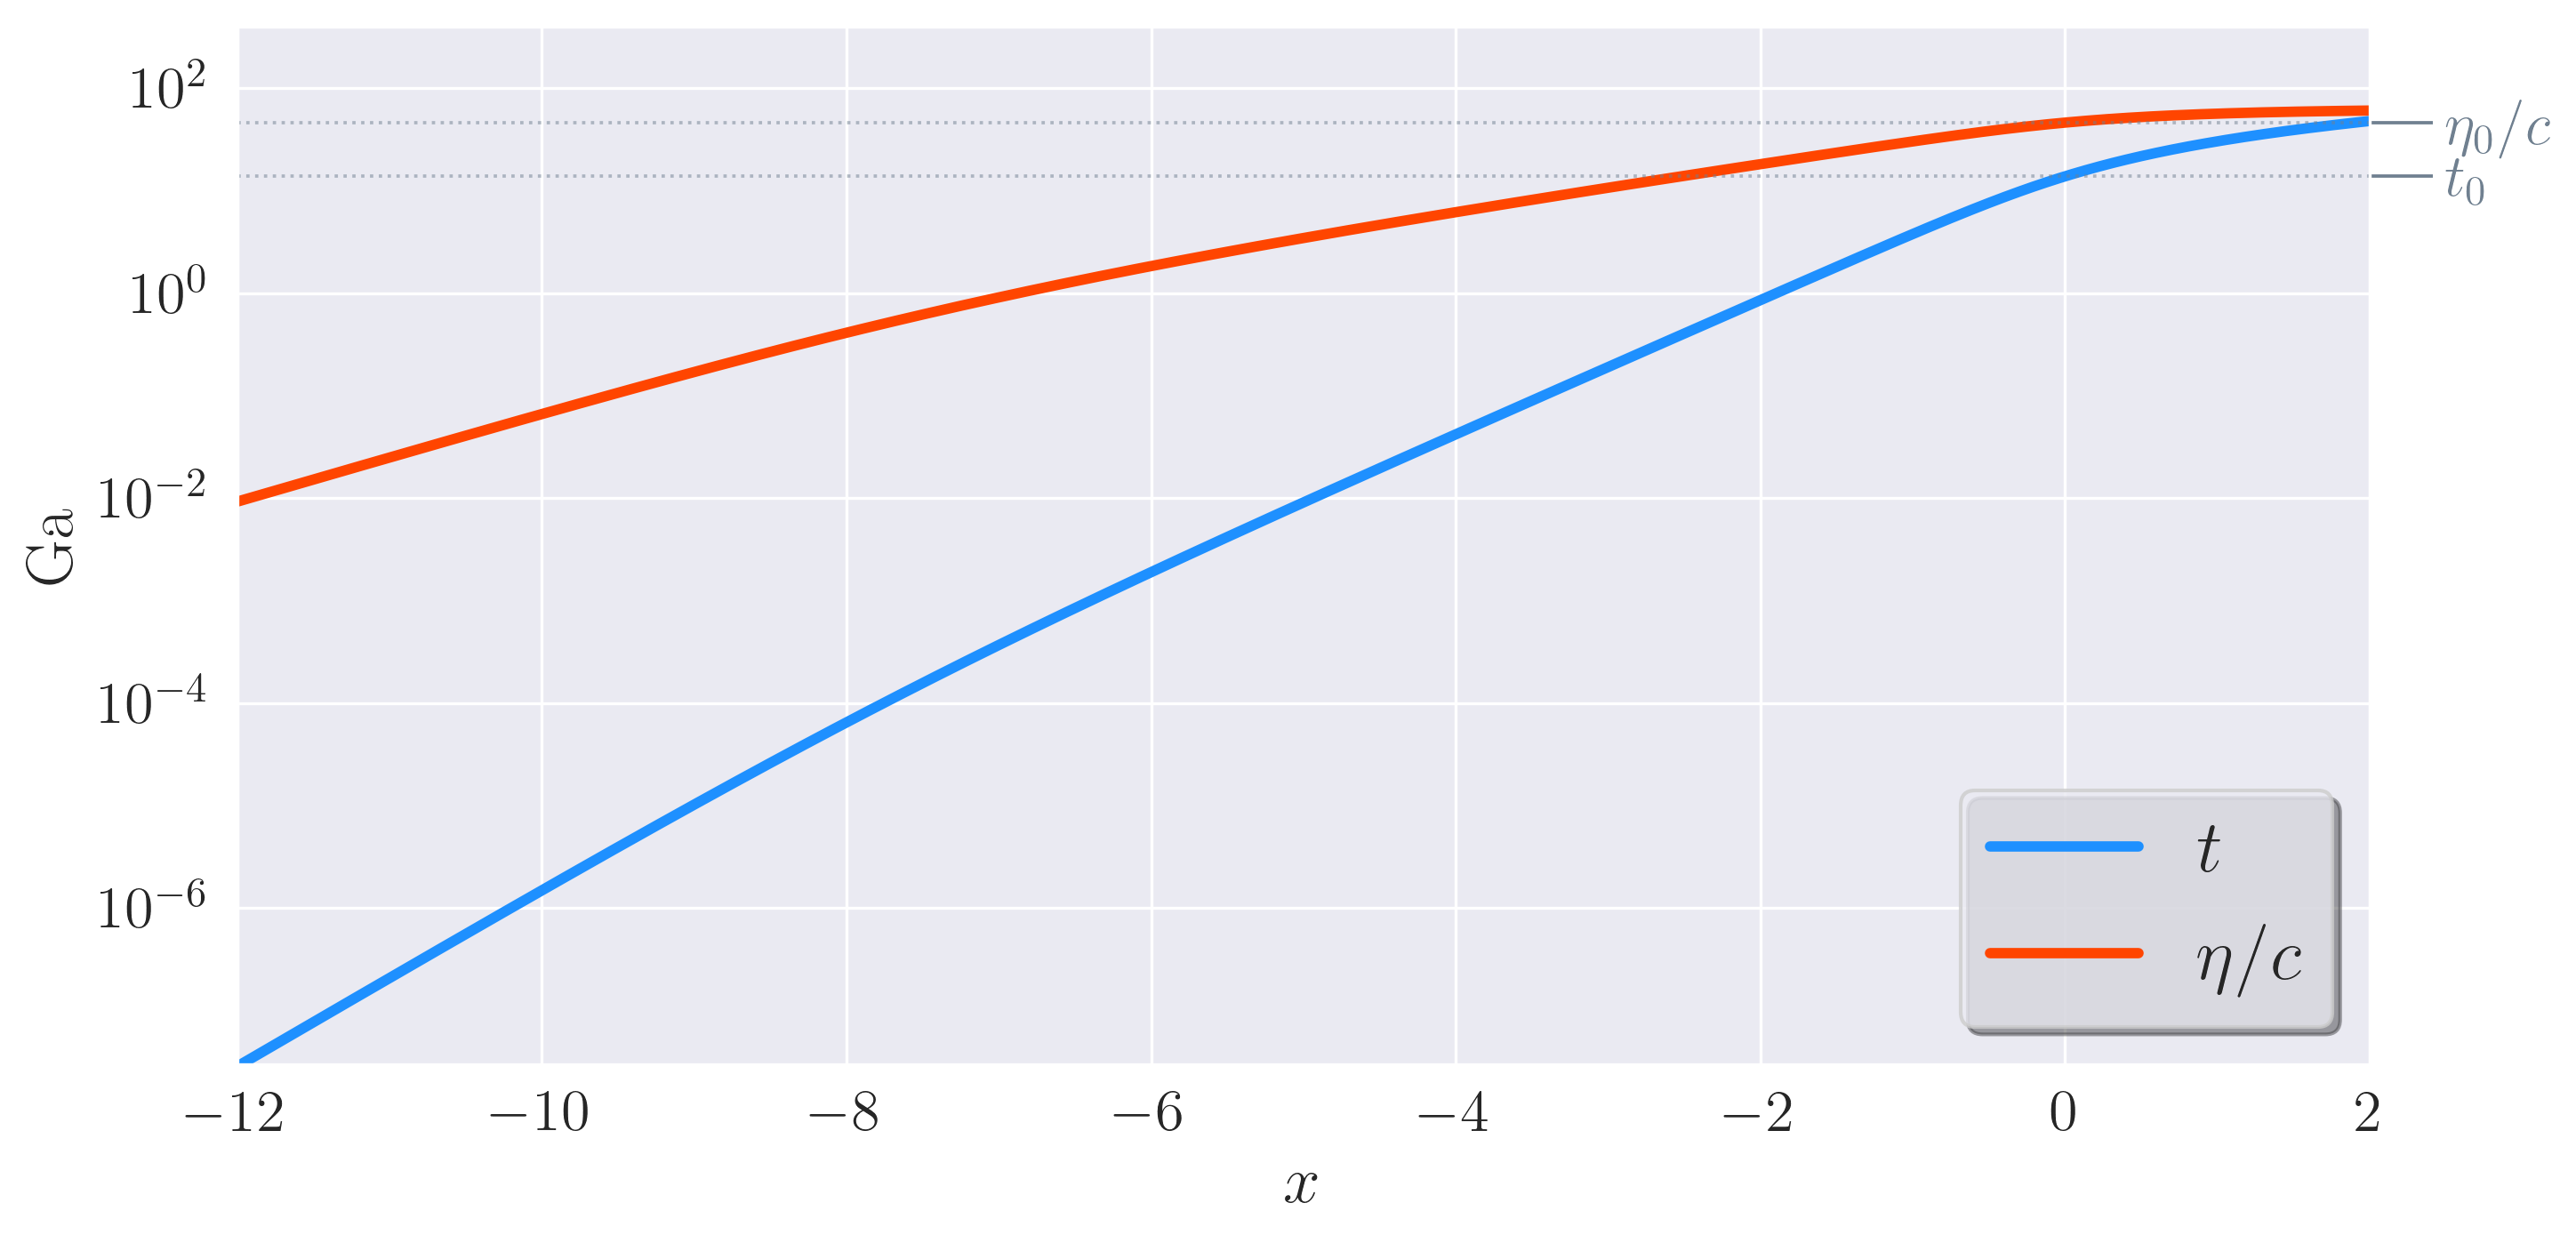
\includegraphics[width=\linewidth]{milestone1/time_measures.png} 
    \caption{Cosmic time $t(x)$ and conformal time per speed of light $\frac{\eta(x)}{c}$. Note the logarithmic $y$-axis.} 
    \label[fig]{mil1:res:fig:conformal_cosmic_time}
\end{figure}

We present the time of various milestones in the history of the universe, given this model, in~\cref{mil1:res:tab:time_of_events} in our main time variable, redshift and cosmic time. 


\begin{table}[h]
    \setlength\tabcolsep{0pt} % let LaTeX figure out amount of inter-column whitespace
    % \begin{tabular*}{\linewidth}{@{\extracolsep{\fill}} l *{3}{d{2.4}} }
    \caption{The values of the logarithmic scale factor $x$, the redshift $z$ and the cosmic time $t$ corresponding to four important milestones in the history of the universe.}
    \label[tab]{mil1:res:tab:time_of_events}
    \begin{tabular*}{\linewidth}{@{\extracolsep{\fill}} l *{1}{d{2.4}} *{1}{d{4.4}} *{1}{d{2.7}} }
    \toprule
    % & \multicolumn{3}{c}{Time of event} \\
    & \multicolumn{1}{c}{$x$} & \multicolumn{1}{c}{$z$} & \multicolumn{1}{c}{$t$} \\
    \midrule
    Rad.-matter equality  & -8.132 & 3400    & 51.06\unit{ka} \\
    Acceleration onset         & -0.4869 & 0.6272 & 7.752\unit{Ga} \\
    Matter-DE equality    & -0.2558 & 0.2915 & 10.37\unit{Ga} \\
    Today                 & -0.000 & 0.000   & 13.86\unit{Ga} \\
    \midrule
    \multicolumn{2}{l}{Conformal time today:} & \multicolumn{2}{c}{$\eta_0 = 46.32 c$~Ga}\\
    \bottomrule
\end{tabular*}
\end{table}



\subsubsection{Supernova fitting}
    Before adjusting any parameters, we compared our initial model with the supernova data from~\citet{supernovadata}. This by-eye comparison is found in~\cref{mil1:res:fig:lum_dist_vs_z}. We demonstrated the model favoured by the data in the same plot.
    
    \begin{figure}[!ht]
        \centering
        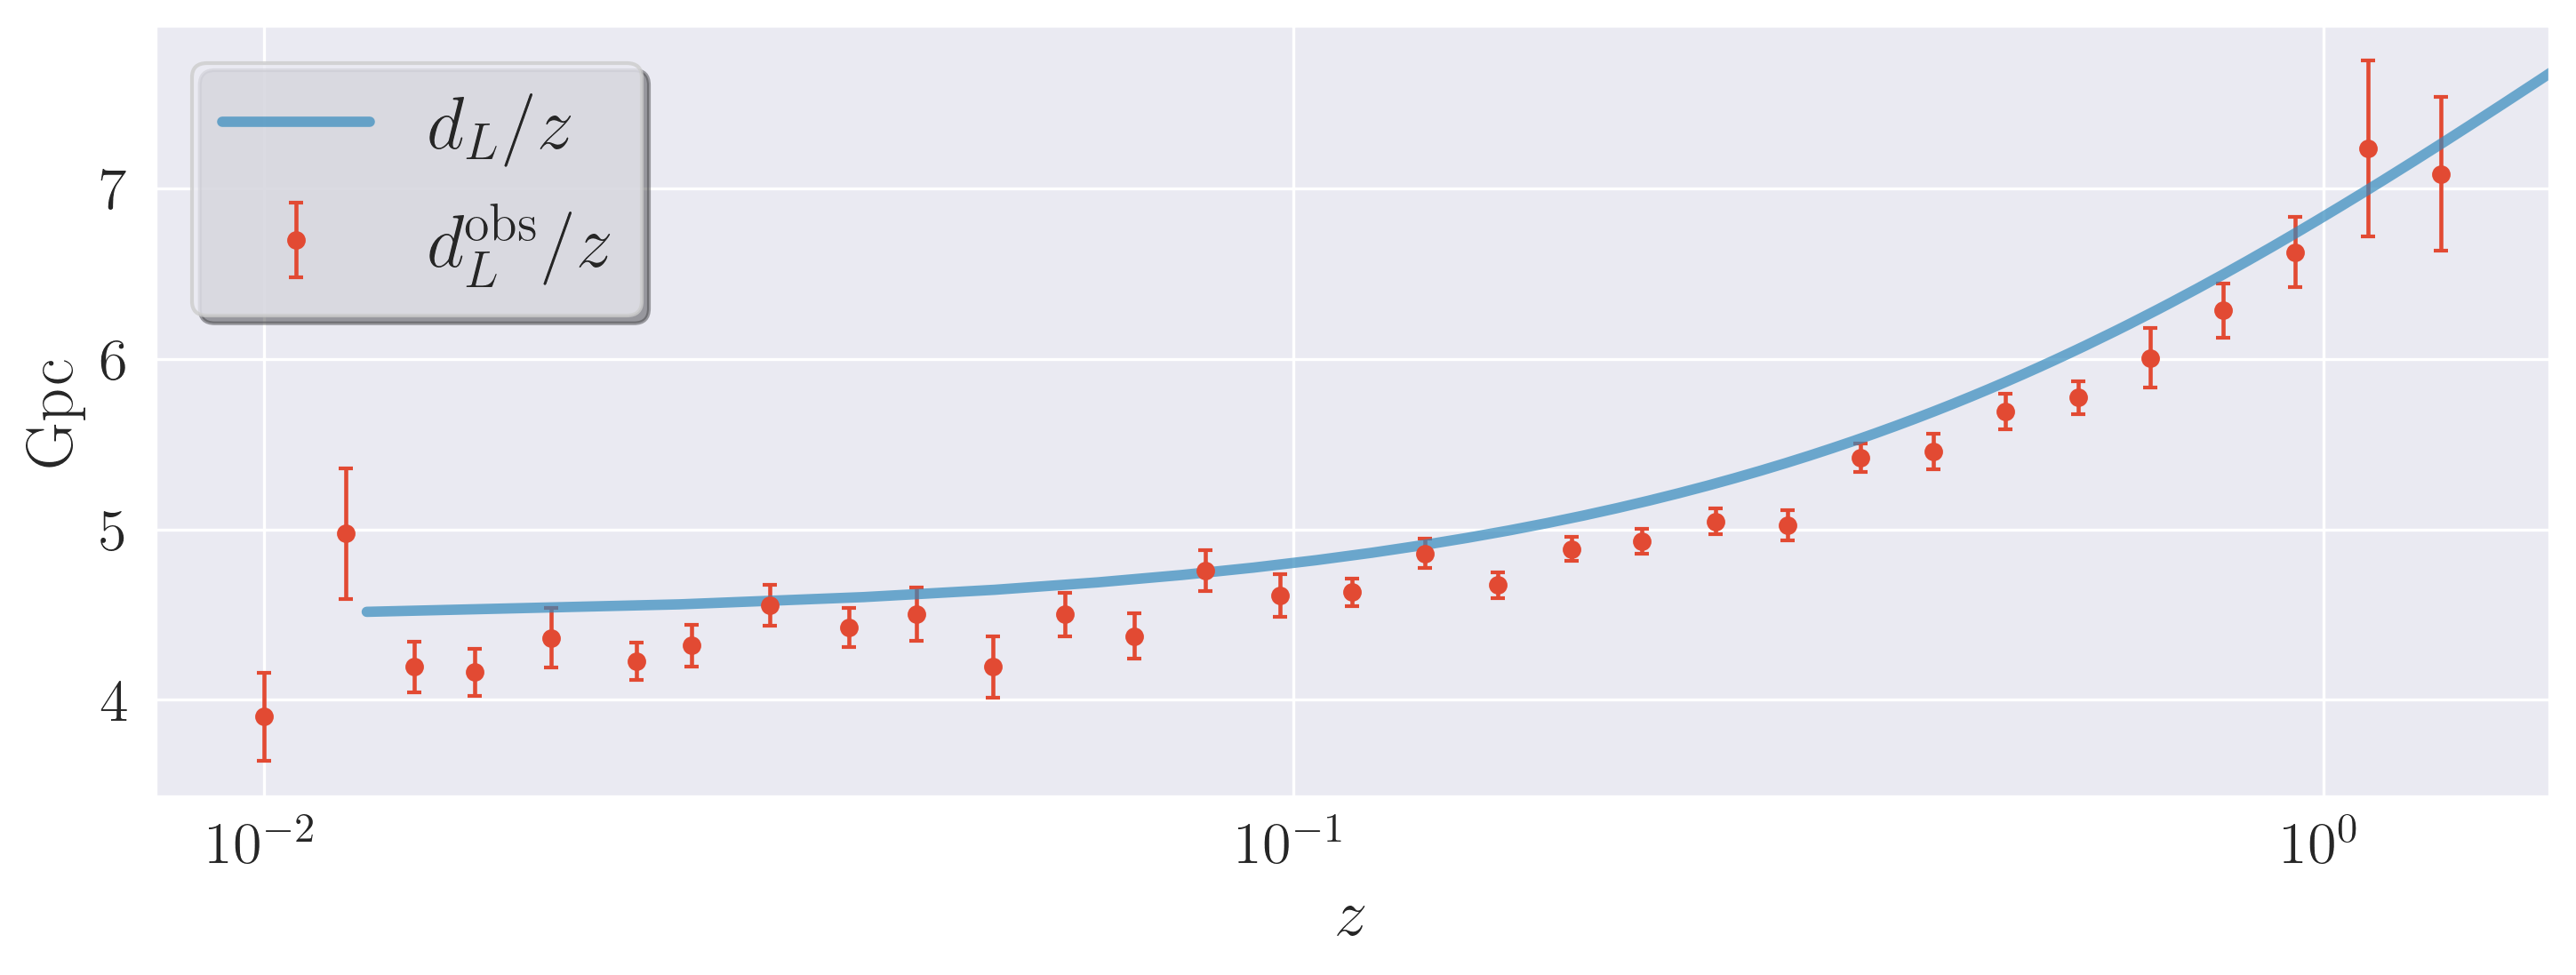
\includegraphics[width=\linewidth]{milestone1/lum_distance_vs_redshift.png} 
        \caption{The observed (dots) and computed (lines) luminosity distance per redshift $\frac{d_L^\mathrm{obs}(z) \pm \sigma_\mathrm{err}(z)}{z}$ and $\frac{d_L(z)}{z}$. The yellow line represents the fiducial model, whilst the green line is the revised model resulting from the MCMC.} 
    \label[fig]{mil1:res:fig:lum_dist_vs_z}
    \end{figure}

    The MCMC yielded $\chi^2_\mathrm{min}=29.28$ for the best-fit. We present confidence regions for $\OmgM$ and $\OmgL$ in~\cref{mil1:res:fig:omega_space} at two levels; 68.4\% and 95.5\%. The distribution of the curvature parameter is shown in~\cref{mil1:res:fig:curvature_pdf}. As for the Hubble constant, the distribution is found in~\cref{mil1:res:fig:hubble_pdf}.
    \begin{figure}
    \begin{subfigure}{\linewidth}
        \centering
        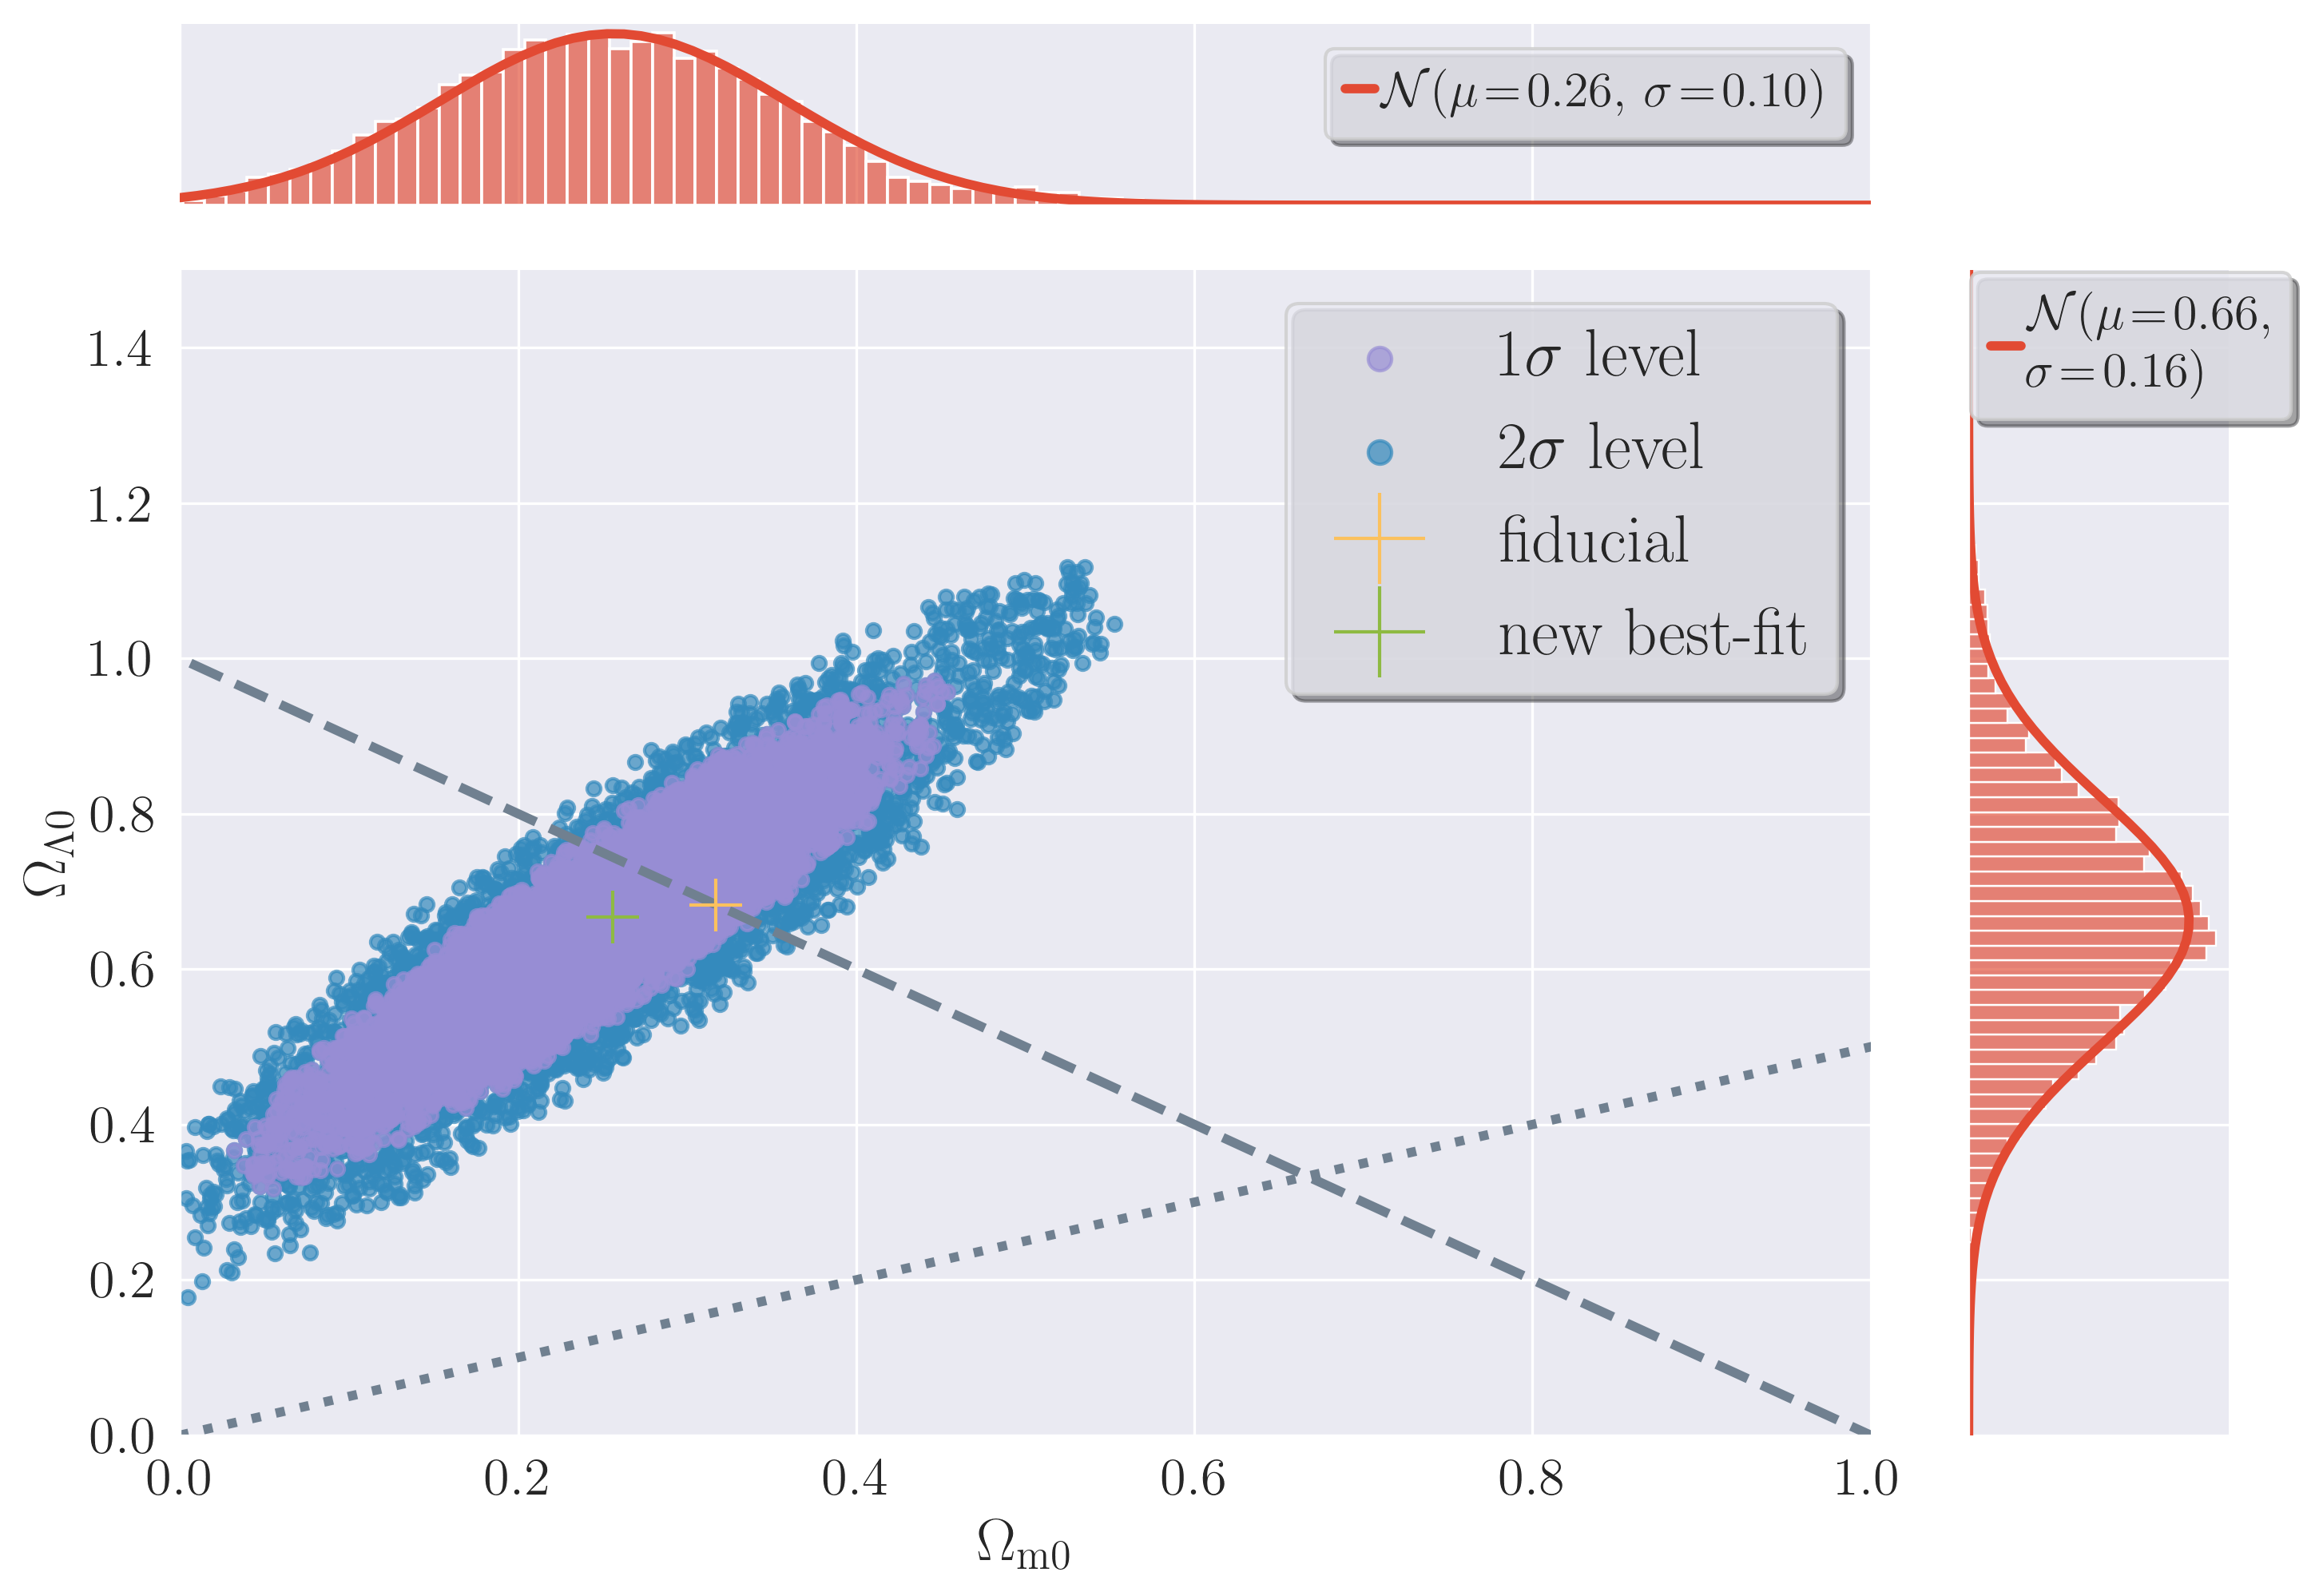
\includegraphics[width=\linewidth]{milestone1/omega_phase_space.png} 
        \caption{The dots give constraints on the parameters that quantify the contribution of matter and cosmological constant to the cosmic energy budget today $(\OmgM,\, \OmgL)$. The Planck parameters from~\cref{mil1:imp:eq:fiducials} and~\cref{mil1:imp:eq:derived_fiducials} and the new best-fit parameters are indicated by crosses. The dashed grey line points to a flat universe; below/above this meaning an open/closed universe. The dotted grey line signifies zero acceleration; below/above indicating a decelerating/accelerating universe. The distributions of the accepted samples of $\OmgM$ and $\OmgL$ are illustrated by the top and right panel, respectively.} 
    \label[fig]{mil1:res:fig:omega_space}
    \end{subfigure}
    \begin{subfigure}{\linewidth}
        \centering
        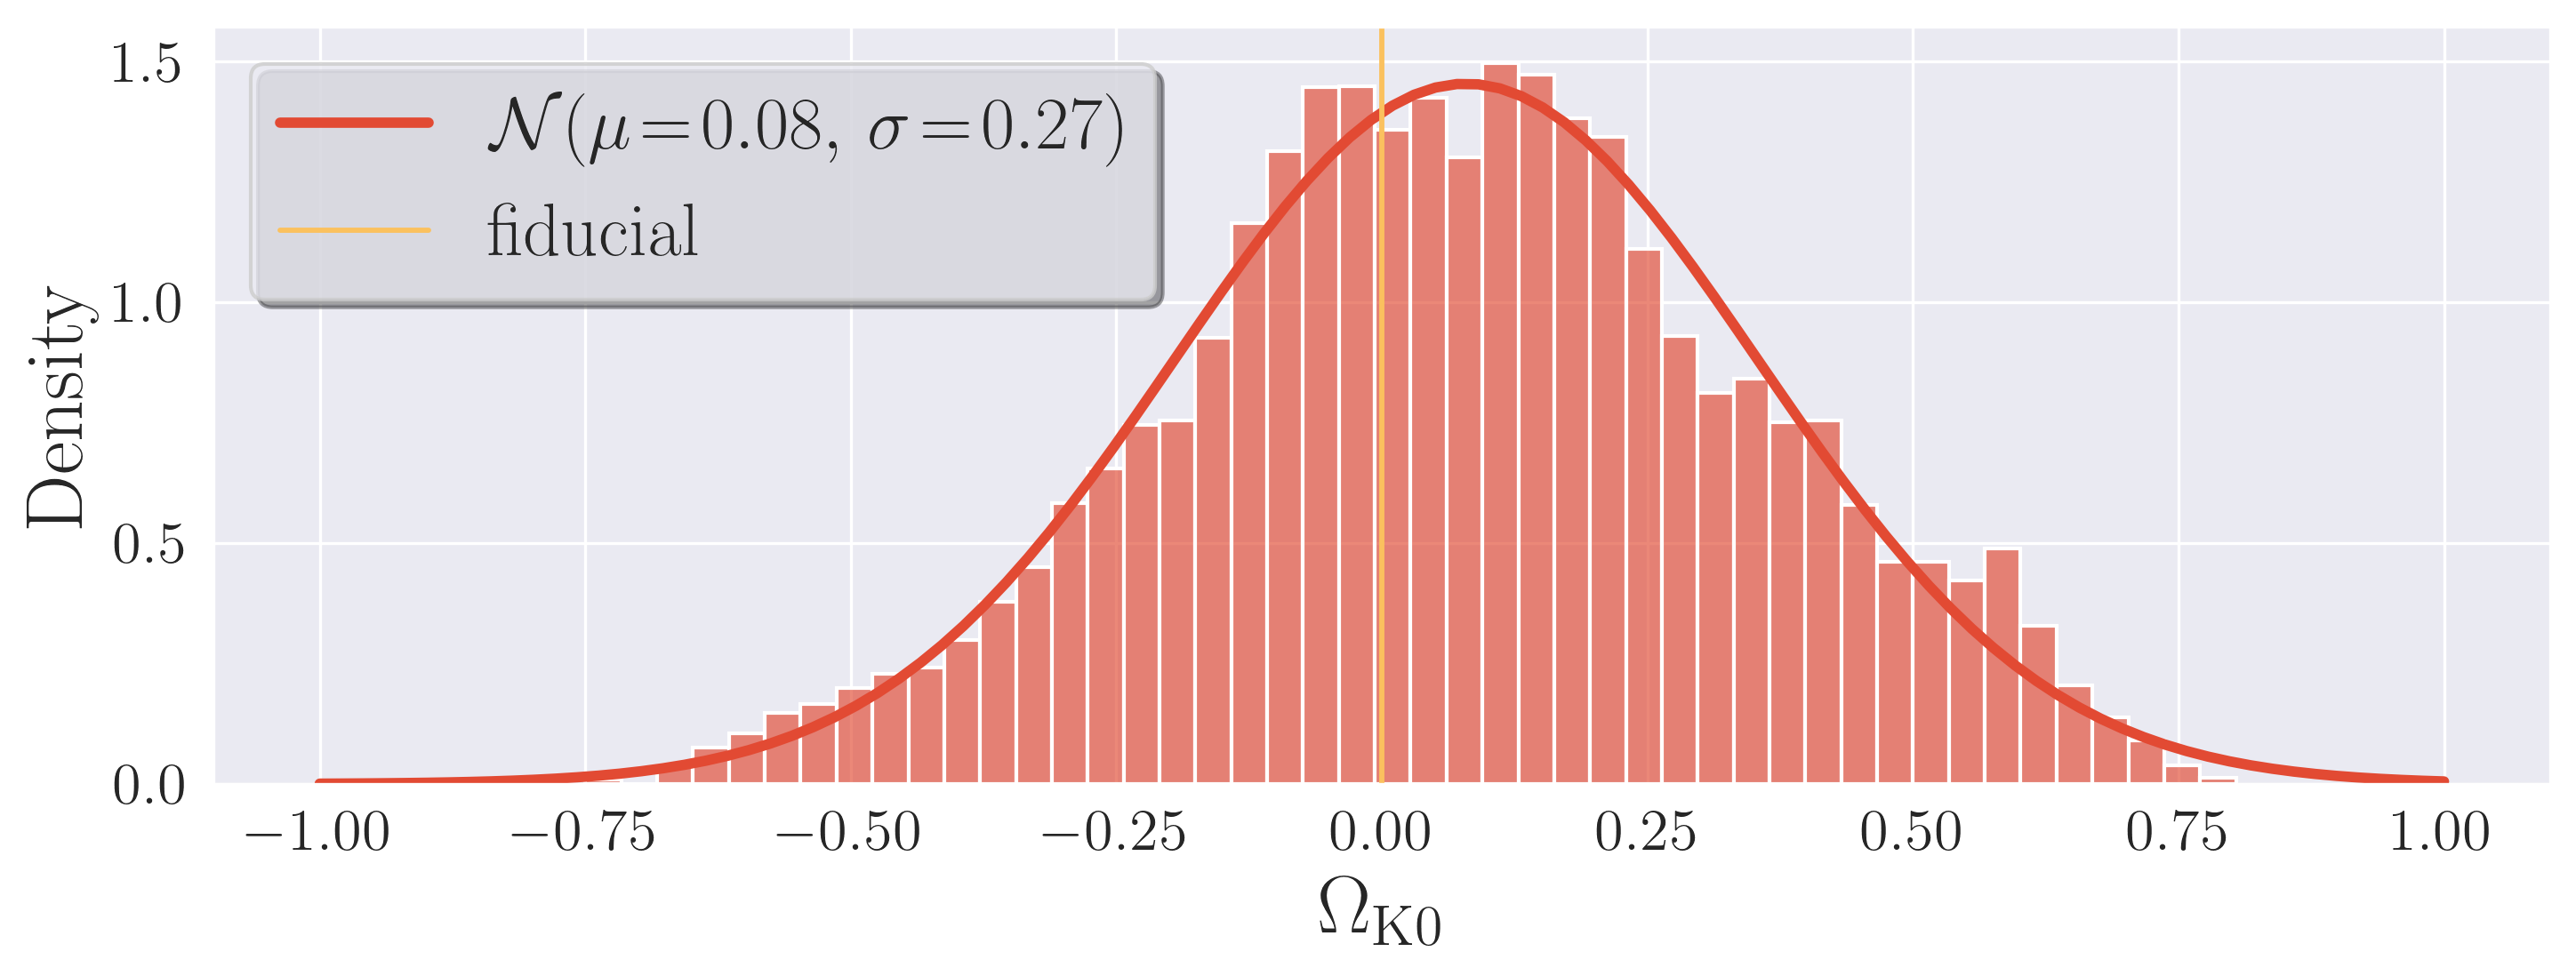
\includegraphics[width=\linewidth]{milestone1/curvature_pdf.png} 
        \caption{Posterior distribution of parameter quantifying the contribution of curvature to the cosmic energy budget today.} 
    \label[fig]{mil1:res:fig:curvature_pdf}
    \end{subfigure}
    \begin{subfigure}{\linewidth}
        \centering
        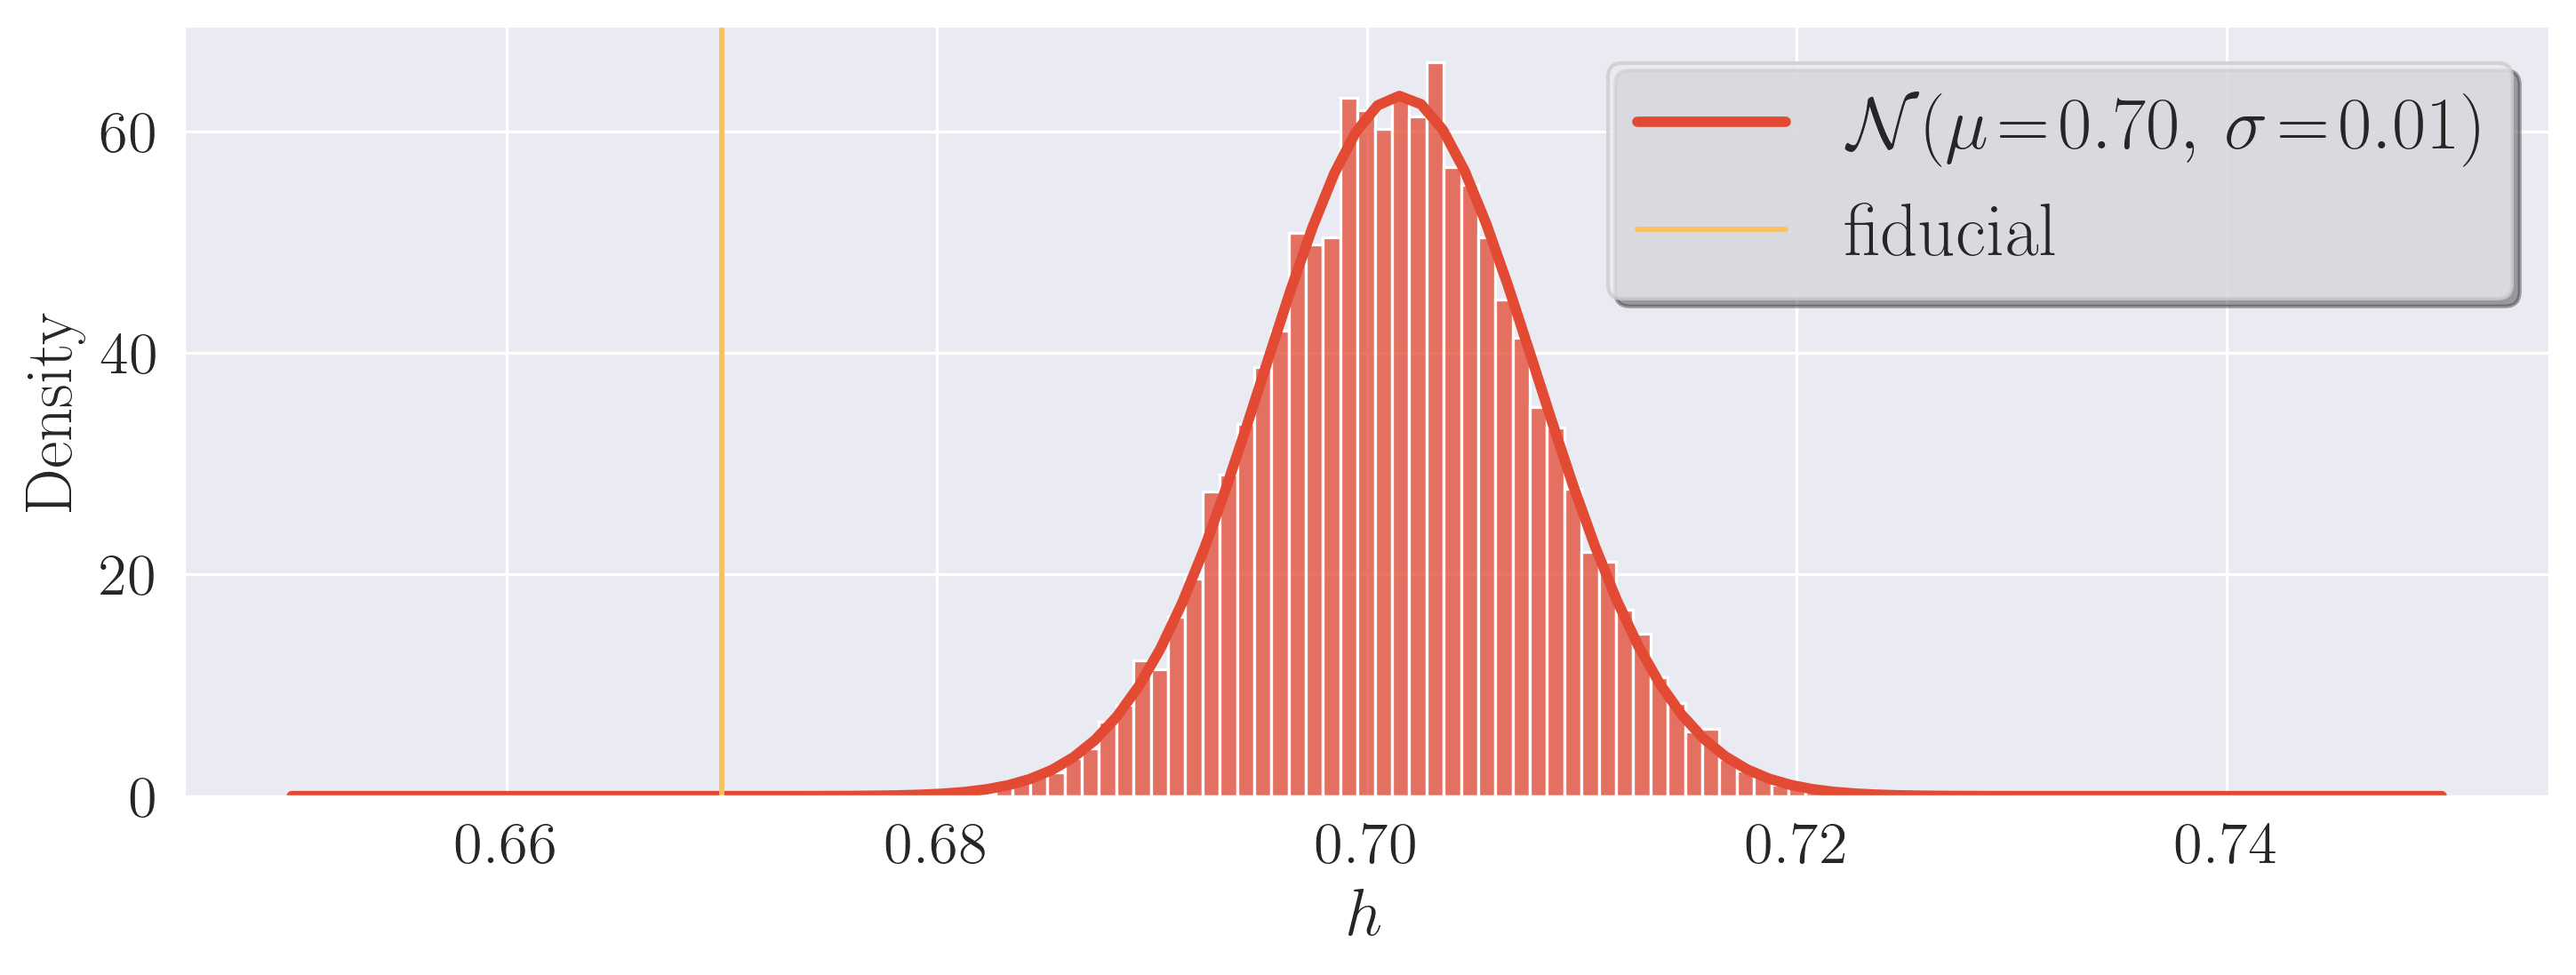
\includegraphics[width=\linewidth]{milestone1/hubble_pdf.png} 
        \caption{Posterior distribution of the Hubble constant $h=H_0$~$[100\text{~km}\text{~s}^{-1}\text{~Mpc}^{-1}]$.} 
    \label[fig]{mil1:res:fig:hubble_pdf}
    \end{subfigure}
    \caption{Results from the MCMC of 10\,000 iterations. The histograms show the distributions of accepted samples and the curves are their PDFs.}
    \label[fig]{mil1:res:fig:mcmc_results}
    \end{figure}
    The distributions were fitted as normal distributions (demonstrated in~\cref{mil1:res:fig:mcmc_results}) $\mathcal{N}(\mu, \sigma)$ with average $\mu$ (best-fit) and standard deviation $\sigma$ (error). We got the following set of new best-fits:
    \begin{equation}
        \begin{split}
            h &= 0.70 \pm 0.01 \\
            \OmgM &= 0.26 \pm 0.10 \\
            \OmgL &= 0.66 \pm 0.16 \\
            \OmgK &= 0.08 \pm 0.25
        \end{split}
    \end{equation}

    